\documentclass[10pt,twocolumn]{article}
\usepackage[margin=0.62in]{geometry}
\usepackage{booktabs}
\usepackage{graphicx}
\usepackage{threeparttable}
\usepackage{amsmath}
\usepackage{amssymb}
\usepackage{microtype}
\setlength{\columnsep}{0.22in}
\setlength{\textfloatsep}{5pt plus 2pt minus 2pt}
\setlength{\floatsep}{4pt plus 2pt minus 2pt}
\setlength{\intextsep}{5pt plus 2pt minus 2pt}
\usepackage{url}
\usepackage{caption}
\usepackage[hidelinks]{hyperref}
\usepackage[numbers,sort&compress]{natbib}
\graphicspath{{figures/}}
\captionsetup{font=small,labelfont=bf}
\title{Source-free pilot adaptation for RIS-assisted wideband MIMO channel estimation under explicit distribution shifts}
\author{Pengliang Tian$^{1}$ \and Changjiang Zhang$^{2,*}$\\[-2pt]
\small $^{1}$Communication and Information Engineering, Beijing University of Posts and Telecommunications Century College, Beijing, China\\
\small $^{2}$Beijing University of Posts and Telecommunications Century College, Beijing, China\\
\small Author contacts: tianpengliang@ccbupt.cn; zhangchangjiang@ccbupt.cn\\
\small ORCID (Pengliang Tian): 0009-0003-5941-9797\\
\small $^{*}$Corresponding author: Changjiang Zhang (zhangchangjiang@ccbupt.cn)}
\date{}

\begin{document}
\maketitle

\begin{abstract}
Learned channel estimators can lose accuracy after deployment when propagation statistics shift and target channel labels are unavailable. We establish an evidence-bounded benchmark for source-free pilot adaptation in an explicit wideband BS--RIS--UE simulator, where RIS size, reflection phases, beam squint, angular displacement and delay scaling are controlled shift factors. A source estimator is updated from received pilots only and scored with target channel state information that is withheld from adaptation. Across four canonical shifts, a lightweight residual adapter reduces NMSE relative to a frozen estimator by 0.83--3.21\%, with corresponding changes in bit-error rate and spectral efficiency; a disjoint support/evaluation protocol preserves the recovery direction. The result is conditional: an eight-element beam-squint cell at 5 dB worsens all three communication-facing outcomes, and least squares (LS) remains competitive. Full-model adaptation is more accurate but updates 115,328 parameters versus 16,576 for the adapter. A preregistered delay-tail objective performs worse than a no-physics control and is therefore retained as a negative control. The study provides a reproducible benchmark for pilot-only recovery, capacity cost and failure boundaries within the tested synthetic generator, rather than a claim of universal superiority.
\end{abstract}

\textbf{Keywords:} reconfigurable intelligent surface; wideband MIMO; source-free adaptation; channel estimation; distribution shift; pilot efficiency.

\section{Introduction}

Channel state information (CSI) is the interface between a wireless propagation environment and almost every downstream decision in a MIMO transmitter or receiver. In a deployment-oriented system, however, CSI is not an abstract input. It must be reconstructed from a finite pilot budget, under a propagation process that can change with user position, blockage, mobility, carrier frequency and hardware configuration. A learned estimator can be very accurate on the source distribution used for training and still become biased when a new environment changes the angular or delay structure of the channel. Obtaining complete target-domain CSI labels to correct that bias would remove much of the practical attraction of a low-overhead learned estimator.

Reconfigurable intelligent surfaces (RISs) make this deployment problem more structured and more difficult. A cascaded BS--RIS--UE link contains a BS-to-RIS response, a configurable reflection response and a RIS-to-UE response. The effective channel is therefore controlled by both geometry and the surface state, while a wideband array introduces frequency-dependent steering. Beam squint makes a single narrowband approximation inadequate when the fractional bandwidth is non-negligible. The same received pilot energy can consequently correspond to different spatial and frequency signatures after a modest change in user position or delay spread. RIS channel-estimation studies have developed model-based, location-aware, dictionary-based and physics-informed approaches, but their evaluation protocols do not always isolate the information used for target adaptation from the information used for final scoring.

Source-free or test-time adaptation offers a natural way to use the pilots that are already present at deployment. The central constraint is that the target channel labels are unavailable. The method can therefore minimize a measurement-consistency objective on received pilots, but it cannot select hyperparameters by looking at the hidden target channel. This distinction matters because a method that improves a reconstruction loss on the same samples used for scoring may be exploiting a test-time fitting opportunity rather than demonstrating transport to a new target block. It also matters for communication metrics: a lower channel-estimation error does not automatically imply lower BER or higher spectral efficiency when the estimator changes the beamforming vector.

This study asks a bounded empirical question. Under explicit wideband RIS distribution shifts, how much recovery can be obtained from pilot-only adaptation of a frozen learned estimator, and how does that recovery depend on geometry, SNR, pilot budget and adaptation capacity? We answer the question with a protocol that exposes the shift factors, separates target support from target evaluation when the strict test is used, reports both channel and communication metrics, and retains non-improving cells. The work is deliberately framed as a benchmark and failure analysis. A tested physical penalty is not promoted to a mechanism unless it makes an independent contribution in a preregistered control.

We therefore make the protocol, rather than a new channel model, the central contribution. The release exposes the RIS-wideband shift factors, separates canonical batch-level adaptation from disjoint support/evaluation, compares adapter-only and full-model updates at matched target observations, and includes LS, fixed-dictionary OMP, pilot-budget sensitivity, failure cells and a negative physical control. This structure makes the recovery claim auditable while keeping its simulator and observation-budget boundary explicit.

The main conclusion is conditional. In the tested explicit-RIS simulator, pilot-only adaptation recovers part of the degradation of a frozen learned estimator across four canonical shifts and retains a downstream communication benefit in that sweep. The benefit is reduced or reversed in particular small-RIS beam-squint cells, and LS can have lower BER. Full-model adaptation buys additional accuracy at a substantially larger trainable parameter count. These observations support deployment decisions about when adaptation is worth its cost; they do not establish universal dominance over classical estimation or a universally valid physical-consistency mechanism.

\section{Related Work and Search Boundary}

\subsection{RIS and wideband channel estimation}

RISs have been studied as programmable propagation structures for wireless communications, with signal-processing formulations that make the surface response part of the end-to-end channel \cite{elmossallamy2020ris,bjornson2022ris}. Channel estimation in this setting must account for the cascaded structure and for the fact that a surface state can be changed between pilot observations. In wideband systems, the frequency dependence of array responses produces beam squint and couples angular and delay information. Recent broadband RIS work considers location or element grouping as a way to reduce the effective estimation burden \cite{broadbandRisEstimation2025}, while wideband multi-RIS work explicitly models OFDM and beam-squint effects \cite{widebandMultiRis2025}. These approaches motivate exposing the propagation factors in the generator rather than using an unspecified channel distribution.

The present study does not claim a new RIS channel model. Its purpose is to make the target shift observable and reproducible at the protocol level. RIS size, beam-squint state, angular shift and delay scaling are stored in the experiment artifacts. The same generator supplies the learned estimator, LS reference, OMP reference and robustness controls. This common generator prevents a baseline from receiving a different propagation problem simply because it is classical or neural.

\subsection{Self-supervised and online adaptation}

Ground-truth-free channel estimation has been explored for IRS-aided communication, including self-supervised objectives that use signal structure rather than complete channel labels \cite{zhang2023selfsupervised}. A recent multi-task self-supervised RIS estimator also addresses time-varying noise and refinement without treating every target channel as a labelled training example \cite{bai2026multitask}. More generally, zero-shot online channel estimation has been proposed for massive MIMO, showing that an estimator can update from deployment observations without a conventional target-label training set \cite{gao2026zeroshot}. These studies establish that label-free refinement is a relevant design space.

The evaluation question here is narrower. We ask whether a frozen learned estimator recovers under an explicit RIS-wideband distribution shift when the update is restricted to received pilots, and whether that recovery survives an evaluation block whose random seed is not available during adaptation. The distinction is between the availability of an unsupervised loss and the independence of the evidence used to claim transport. We therefore report both a canonical per-batch adaptation sweep and a strict held-out support/evaluation experiment instead of treating them as interchangeable.

\subsection{Physics-informed and adaptive model-based methods}

Physics-informed RIS estimation and digital-twin formulations incorporate propagation structure into the estimator or simulator \cite{hybridPhysicsRis2026,han2025digitaltwin}. Sparse and dictionary-adaptive methods provide classical or hybrid references for mmWave RIS links \cite{adaptiveRisGlobecom2024,superResolutionRis2026}. Unified XL-RIS estimators extend the scale of the array model and address multi-user settings \cite{unifiedXlRis2024}. These contributions are complementary to the benchmark here. They clarify which structures can be encoded, but they do not by themselves establish how a source-trained estimator should be adapted from unlabeled target pilots or where the resulting gain fails.

Our preregistered control is designed to keep this distinction explicit. A first-difference term and a delay-tail term are evaluated against a no-physics pilot-consistency adapter on held-out target blocks. If a term does not improve the hidden CSI under the paired analysis, it is recorded as a negative control. This prevents a physical interpretation from being inferred solely because a term has a plausible name or because it lowers the adaptation objective.

\subsection{Positioning and search boundary}

The related-work search covered the five DOI-verified neighboring records summarized in Supplementary Table~S1, as well as additional recent records on self-supervised RIS estimation, zero-shot online estimation, wideband beam squint and digital twins. The search was performed against publisher, Crossref and metadata services in October 2026. Some broad keyword endpoints were rate limited or protected by anti-bot controls, and no search can certify the absence of an unpublished or differently worded overlap. The positioning claim is consequently search-bounded. The specific protocol-level distinction is the joint reporting of source-free pilot adaptation, explicit wideband RIS shifts, hidden target evaluation, downstream communication metrics, trainable-parameter cost and retained failure cells.

For readability, the full five-record comparison is supplied as Supplementary Table~S1 rather than as a main-text display. Its role is traceability, not a quantitative meta-analysis: ``not confirmed'' records the boundary of the checked metadata and does not assert that a neighboring paper lacks a property. The main-text distinction is therefore the protocol and evidence chain described above, while the supplementary matrix preserves the search record for inspection.

\section{System Model and Evaluation Protocol}

\subsection{Cascaded wideband channel}

Let $K$ denote the number of subcarriers, $N_{\rm t}$ the number of BS transmit antennas and $N_{\rm r}$ the number of RIS elements. For subcarrier $k$, the effective channel is represented by
\begin{equation}
 H_k = h_{\rm UE,k}^{\mathsf T} \Phi h_{\rm BS,k},
\end{equation}
where $h_{\rm BS,k}\in\mathbb{C}^{N_{\rm r}\times N_{\rm t}}$ is the BS-to-RIS response, $h_{\rm UE,k}\in\mathbb{C}^{N_{\rm r}}$ is the RIS-to-UE response and $\Phi=\operatorname{diag}(\rho_1e^{\mathrm j\phi_1},\ldots,\rho_{N_{\rm r}}e^{\mathrm j\phi_{N_{\rm r}}})$ is the fixed reflection response for one realization. Here $h_{\rm UE,k}^{\mathsf T}$ is a transpose without complex conjugation, matching the row-vector contraction implemented by the released generator. The simulator uses a small number of independent paths on each hop. Each path contributes a complex gain, a delay phase $\exp(-\mathrm j2\pi f_k\tau)$ and a normalized array response. With beam squint enabled, the spatial frequency of the array response is multiplied by a subcarrier-dependent spacing factor. With beam squint disabled, the spacing factor is fixed across subcarriers.

The generator is intentionally compact rather than a claim of hardware-level fidelity. It makes the variables that define the shift visible: RIS elements are set to 8, 16 or 32 in robustness experiments; angular offsets are 0.04, 0.08, 0.12 or 0.18; delay scales are 1.2, 1.4, 1.6 or 2.0; and the beam-squint switch is recorded. The canonical setting uses $K=16$, $N_{\rm t}=4$, $N_{\rm r}=16$, three BS-side paths and two UE-side paths. The reflection phases are sampled per realization and remain fixed while the receiver observes the pilot block. The subcarrier coordinate is normalized to $f_k\in[-0.5,0.5)$; no physical carrier frequency, bandwidth or subcarrier spacing is assigned. Delays are normalized uniforms on $[0,0.25]$ and $[0,0.20]$ before delay scaling, path gains are normalized by path count, and no explicit path-loss, mutual-coupling or physical-aperture model is included. Thus $N_{\rm r}$ is an element-count factor in this release, not a calibrated aperture size.

\subsection{Pilot observation and target shifts}

For a pilot matrix $P\in\mathbb{C}^{N_{\rm t}\times N_{\rm p}}$, the observation at subcarrier $k$ is
\begin{equation}
 Y_k = H_kP + W_k,
\end{equation}
where $N_{\rm p}$ is the pilot count and $W_k$ is circular complex Gaussian noise calibrated to the channel power and the requested SNR. The canonical protocol uses the first two columns of the identity matrix as pilots and 15 dB SNR. The LS reference fills the observed antenna columns with $Y_k$ and sets the unobserved columns to zero. This is a deliberately transparent reference for the low-pilot regime, not an oracle estimator with knowledge of the unobserved channel.

The source domain uses zero angular shift and unit delay scale. A target shift changes the angle distribution and delay scale while retaining the same generator, number of subcarriers and pilot operator. The four canonical pairs are $(0.04,1.2)$, $(0.08,1.4)$, $(0.12,1.6)$ and $(0.18,2.0)$. Source training uses 4,096 labelled realizations and 12 AdamW epochs with batch size 128. A source validation block contains 512 realizations. The canonical target sweep contains 512 target realizations for each shift and seed. In the stricter held-out protocol, a 512-realization support block and a separate 512-realization evaluation block are generated with disjoint seed ranges for each shift.

Figure~\ref{fig:protocol} summarizes the information flow. Source CSI is used only to train the source estimator. The target adapter receives pilot features from the support block, while the target evaluation CSI is held back until scoring. The target labels may be present in the output artifact because they are needed to calculate NMSE, BER and spectral efficiency, but the adaptation optimizer does not receive them.

The protocol was locked before the final comparison artifacts were generated. In particular, the source estimator, target shifts, pilot operator, adapter update count, loss weights, seed list and primary outcome were fixed in the experiment manifests. The canonical sweep and the held-out test are therefore interpreted as different estimands. The sweep measures whether a target-time update can move a reconstruction in the intended direction when the target batch supplies the unlabeled support. The held-out test measures whether an update fitted on one target block transfers to another block from the same shifted generator. Keeping these estimands separate avoids using the stronger held-out language for the more permissive batch-level result.

\begin{figure*}[t]
\centering
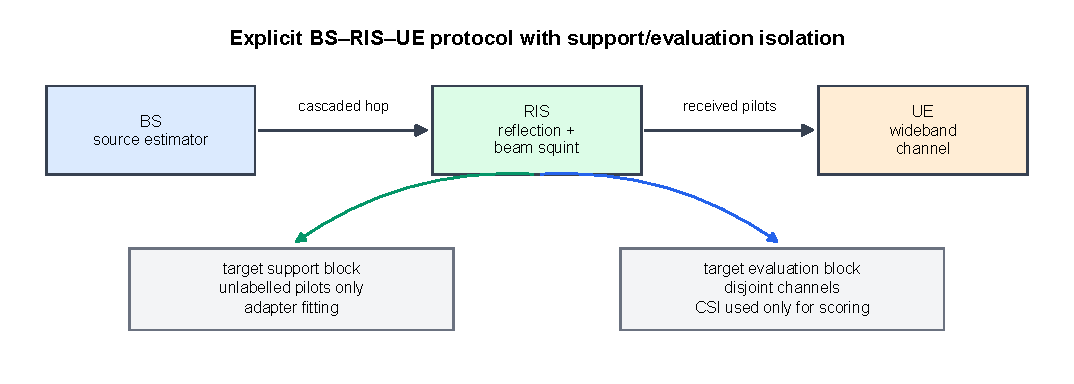
\includegraphics[width=0.98\textwidth]{fig1_protocol.pdf}
\caption{\textbf{Explicit BS--RIS--UE protocol and label isolation.} The source estimator is trained with source CSI. At target time, received pilots enter either a canonical batch-level adapter or a support-fitted adapter. In the strict evaluation, the support and evaluation blocks use disjoint random seeds and channel realizations. Target CSI in the evaluation block is used only to calculate the reported metrics.}
\label{fig:protocol}
\end{figure*}

\subsection{Source estimator and source-free adapter}

The source estimator is a compact real-valued multilayer perceptron. Complex pilot observations are represented by concatenating real and imaginary parts. The network maps $2KN_{\rm p}$ input features to $2KN_{\rm t}$ output features through two 256-unit GELU hidden layers. It is trained with a supervised mean-squared error on the source channel. No target CSI is used in this training stage.

The lightweight adapter is a residual network with a 64-unit GELU hidden layer and a zero-initialized final linear layer. For a frozen estimate $z=f_\theta(Y)$, the adapted estimate is
\begin{equation}
 \tilde z = z + r_\phi(z).
\end{equation}
Zero initialization makes the initial adapter equal to the frozen estimator, so any change is attributable to the target update rather than a randomly initialized replacement model. The adapter has 16,576 trainable parameters. It is updated for ten Adam steps with learning rate $10^{-3}$.

The pilot-consistency objective is
\begin{equation}
 \mathcal L_{\rm pc}=\|S\tilde H-Y\|_2^2+\lambda_s\|\Delta_f\tilde H\|_2^2+\lambda_p\|\tilde H\|_2^2,
\end{equation}
where $S$ selects the observed pilot columns, $\Delta_f$ is a first-order frequency difference, and $\lambda_s=0.003$ and $\lambda_p=0.1$ are fixed in the recorded configuration. The first-difference term is described as a stabilizing regularizer, not as a proved physical mechanism. The no-physics control sets $\lambda_s=0$. The delay-tail control uses a separate high-delay penalty and is tested only in the preregistered negative-control analysis.

Two adaptation protocols are reported. In the canonical shift sweep, each target block is processed by a prequential batch-level update: 512 target samples form four ordered batches of 128, ten optimizer steps are taken on each batch's pilot features, the adapter state is carried to the next batch, and the post-update prediction for that batch is scored only after optimization. The hidden target CSI is never passed to the optimizer. In the held-out protocol, the adapter is fitted once on the support features and then applied to the separate evaluation block. The second protocol is the stronger test of transport and is the basis for the label-isolation claim.

The distinction between the protocols is operational rather than rhetorical. In the
canonical sweep, the target batch supplies the unlabeled observations used to move
the adapter and also defines the immediate post-update score. This setting measures
whether the pilot objective can repair a target-time estimate under a fixed update
budget. It is useful for exposing the response to progressively stronger shifts,
but it does not by itself establish transfer to new target realizations. The strict
protocol removes that ambiguity by fixing the adapter after support-block updates
and withholding every evaluation pilot and channel label until scoring. The support
and evaluation blocks use disjoint seed ranges while retaining the same generator,
pilot operator and shift parameters. Thus, the held-out analysis tests transfer
within a specified shifted population, whereas the canonical analysis maps the
operating envelope of the update. We report both estimands because collapsing them
would either overstate the batch-level result or hide the deployment-relevant
response to shift magnitude.

\subsection{Classical references and capacity control}

LS is included in every canonical shift and held-out evaluation. To add a sparse classical reference, we construct a fixed transmit-array dictionary with 64 uniformly spaced angle atoms and use complex OMP with a sparsity level of three. The dictionary is frequency-dependent when beam squint is enabled, but it is not adapted to target CSI. OMP is evaluated at two and four identity pilots on the same explicit RIS generator. It is therefore a reference for operating regime and pilot budget, not an implementation of the proposed adapter.

Full-model adaptation updates all 115,328 estimator parameters using the same pilot-only loss and target observations. The comparison is intentionally asymmetric in capacity because deployment decisions often involve choosing between a small update module and updating the whole estimator. We report the parameter count and local CPU wall-clock measurements alongside accuracy. Runtime is treated as a hardware-specific observation, not as a platform-independent speed claim.

\subsection{Metrics and communication evaluation}

For an estimate $\widehat H$ and target $H$, the channel metric is
\begin{equation}
 \operatorname{NMSE}(\widehat H,H)=\frac{\|\widehat H-H\|_2^2}{\|H\|_2^2}.
\end{equation}
Downstream communication is evaluated by QPSK transmission with estimate-based maximum-ratio transmission. The BER is calculated by comparing the recovered real and imaginary bit signs. Spectral efficiency is calculated as the mean of $\log_2(1+|g_k|^2/\sigma_k^2)$ using the true effective gain and the beam formed from the estimated channel. These metrics are not used to choose an adapter or tune a hyperparameter. They are reported to test whether an NMSE change has a communication-facing consequence.

\subsection{Replication, uncertainty and reproducibility}

The independent replication unit is the training/data seed. The fixed seeds are 20261002, 20261003 and 20261004. Within each seed, all methods use matched target realizations, so adapter-versus-frozen and adapter-versus-LS comparisons are paired at the channel-realization level. Seed-level means and standard deviations are reported separately and are not treated as independent samples in a pooled significance claim. For paired evaluation blocks, uncertainty is estimated with 2,000-resample percentile bootstrap intervals and a two-sided Wilcoxon signed-rank test. These intervals and tests are block-conditional summaries of channel-level paired differences, not simulator-independent inference; the 3,072 channel pairs in the physical control are not 3,072 independent experiments. Four shifts, three communication outcomes, 18 robustness cells and multiple controls are therefore reported primarily as effect-size and descriptive evidence. The preregistered delay-tail contrast retains confirmatory wording because its direction and gate were fixed before analysis. The exact paired unit, test, resampling count and seed are written to the JSON artifact. No p-value is used to convert a small numerical difference into a mechanism claim.

The reporting hierarchy follows the experimental unit. Seed-level means and standard deviations describe reproducibility across independent training/data realizations, whereas the bootstrap intervals describe paired variation within a held-out evaluation block. The two summaries answer different questions and are not substituted for one another. No observations were removed after inspecting hidden CSI, and no target label was used to select the adapter, choose a shift, or tune the communication metrics. The detailed seed-by-shift intervals and the full 18-cell robustness matrix are retained in Supplementary Tables~S2 and S3; the main text keeps the primary effect and the edge cell that changes its interpretation.

All table values are generated by Python exporters from JSON artifacts. The figure script reads the same artifacts and emits PDF, SVG and 600-dpi TIFF files. The verification manifest checks the expected artifact set, records the device reported by each run and checks that target labels were not used by the adapter. The final package excludes private host details and credentials. This separation between source data, result summaries and presentation files is part of the reproducibility protocol.

\section{Results}

\subsection{The explicit generator exposes the target shift}

The generator gate confirms that the simulator contains a cascaded BS--RIS--UE response, configurable reflection phases and an explicit beam-squint switch. The same identity-pilot observation operator is used by LS, OMP and the neural methods. The canonical source model reaches a source-validation NMSE of approximately 0.48 across the recorded runs. When the source model is frozen and evaluated under a target shift, its NMSE increases with the strongest angle and delay change, reaching 0.5482 at $(0.18,2.0)$ in the three-seed shift summary. This establishes the evaluation problem before adaptation is considered: the target is not simply a second draw from the source distribution.

The protocol also separates two different sources of apparent improvement. A canonical shift result asks whether an adapter can reduce error after seeing unlabeled pilots from the target batch. The held-out result asks whether the same update fitted on a support block transfers to a disjoint evaluation block. We present the canonical sweep first because it maps the response over four shift levels, then use the held-out experiment as the stronger isolation test.

This ordering is also a guard against a common evaluation ambiguity. If the same target examples are used both to optimize a residual adapter and to report its error, the result is a valid description of batch-level adaptation but it does not by itself establish transport to unseen target realizations. Conversely, a held-out block without the canonical sweep would provide a clean transfer test but would hide how the response changes across the shift axis. Reporting both allows the reader to separate the existence of a usable pilot signal from the strength and stability of the resulting transport claim.

\subsection{Pilot-only adaptation recovers part of the frozen-estimator loss}

Across the four canonical shifts, the adapter has lower NMSE than the frozen estimator in all four rows of Table~\ref{tab:r014}. The absolute recovery is modest at the smallest shift, where the frozen NMSE is 0.4798 and the adapted NMSE is 0.4759, and increases as the frozen estimator becomes less reliable. At $(0.18,2.0)$ the corresponding values are 0.5482 and 0.5306. Expressed relative to the frozen estimate, the reductions are 0.83\%, 1.16\%, 1.91\% and 3.21\% across the ordered shifts. The pattern supports recovery of a learned estimator under the tested shift family, but the percentages should not be read as a universal scaling law.

The communication metrics follow the same direction in this canonical sweep. Adapter BER is lower than frozen BER by 0.00293, 0.00374, 0.00372 and 0.00747, respectively. Spectral efficiency increases by 0.0014, 0.0035, 0.0153 and 0.0378 bit/s/Hz. The communication effect is therefore visible but small in the mild-shift rows and larger at the strongest tested shift. LS is retained in the same table and figure for all three outcomes: its channel NMSE is around 0.514--0.517 and its BER is around 0.0053--0.0060, so it remains a strong BER reference, particularly when the pilot operator is well conditioned. The proper conclusion is that the adapter recovers a learned estimator, not that it replaces a well-conditioned classical estimate in every regime.

Figure~\ref{fig:shift} places these results on a common shift axis. The three panels use the same seed-level mean and standard-deviation convention. The NMSE panel shows the frozen-estimator crossover at the strongest shift, while the BER and spectral-efficiency panels show a consistent adapter direction in the canonical sweep. The figure is a compact evidence unit: the shift creates the performance loss, the adapter reduces part of that loss, and LS remains a separate reference rather than a hidden tuning target.

\begin{figure*}[t]
\centering
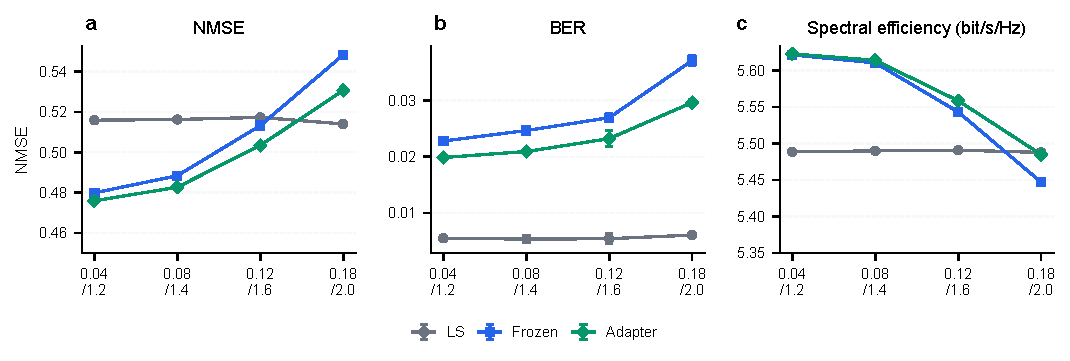
\includegraphics[width=0.98\textwidth]{fig2_shift_sweep.pdf}
\caption{\textbf{Canonical source-to-target shift sweep.} Means and seed standard deviations are shown for three fixed seeds. The x-axis labels give angle shift and delay scale. LS, frozen and adapted estimates are shown for NMSE, BER and spectral efficiency; the same matched target realizations are used for each method. Lower NMSE and BER are better, whereas higher spectral efficiency is better.}
\label{fig:shift}
\end{figure*}

\begin{table*}[t]
\centering
\caption{Explicit-RIS shift sweep. Values are mean (SD) across three CPU seeds.}
\label{tab:r014}
\resizebox{\textwidth}{!}{%
\begin{tabular}{ccrrrrrrrrr}
\toprule
Angle & Delay & LS NMSE & Frozen NMSE & Adapted NMSE & LS BER & Frozen BER & Adapted BER & LS SE & Frozen SE & Adapted SE\\
shift & scale & & & & & & & (bit/s/Hz) & (bit/s/Hz) & (bit/s/Hz)\\
\midrule
0.04 & 1.2 & 0.5159 (0.0002) & 0.4798 (0.0007) & 0.4759 (0.0006) & 0.0055 (0.0001) & 0.0228 (0.0003) & 0.0199 (0.0002) & 5.4885 (0.0003) & 5.6212 (0.0016) & 5.6226 (0.0018)\\
0.08 & 1.4 & 0.5162 (0.0001) & 0.4883 (0.0005) & 0.4827 (0.0004) & 0.0053 (0.0005) & 0.0247 (0.0004) & 0.0209 (0.0002) & 5.4898 (0.0004) & 5.6103 (0.0025) & 5.6138 (0.0014)\\
0.12 & 1.6 & 0.5172 (0.0001) & 0.5132 (0.0004) & 0.5034 (0.0007) & 0.0054 (0.0009) & 0.0269 (0.0007) & 0.0232 (0.0015) & 5.4909 (0.0008) & 5.5432 (0.0002) & 5.5585 (0.0027)\\
0.18 & 2.0 & 0.5140 (0.0001) & 0.5482 (0.0007) & 0.5306 (0.0006) & 0.0060 (0.0005) & 0.0371 (0.0009) & 0.0296 (0.0004) & 5.4877 (0.0006) & 5.4471 (0.0005) & 5.4848 (0.0007)\\
\bottomrule
\end{tabular}
}
\end{table*}


\subsection{The classical baseline depends strongly on pilot budget}

The explicit-RIS OMP experiment supplies a classical reference that is matched to the same generator rather than to a simpler generic channel. Table~\ref{tab:r032omp} and Fig.~\ref{fig:classical} show the mean NMSE across three seeds at 15 dB SNR. With two pilots, LS ranges from 0.5161 to 0.5193 across the four shifts, whereas fixed-dictionary OMP ranges from 0.5590 to 0.5711. With four pilots, both references improve sharply because all four transmit-antenna columns are observed by the identity operator. LS then ranges from 0.0316 to 0.0318 and OMP from 0.0330 to 0.0352.

This result has two implications for the benchmark. First, a sparse prior is not automatically helpful at the smallest pilot budget. The fixed dictionary and the three-atom constraint can be mismatched to the cascaded channel even though the generator is built from a small number of paths. Second, pilot count changes the inverse problem itself. Comparing a two-pilot neural estimator with a four-pilot classical estimate would confound method and observation budget, so the robustness experiment keeps the neural input dimension fixed and reports pilot sensitivity for LS and OMP separately. The OMP run is consequently used to delimit the baseline regime rather than to manufacture a stronger claim for the adapter.

The four-pilot result is useful as a conditioning check rather than as a competing headline. When all four transmit-antenna columns are observed, the identity operator removes the missing-column ambiguity that defines the two-pilot setting, and both classical references approach the channel error floor of this compact simulator. The experiment therefore makes the observation budget explicit. It also prevents a favorable interpretation of the neural result that would arise simply from comparing a learned model with a classical method under different information constraints. Supplementary source data retain the seed-level values used for the bars and the table.

\begin{figure*}[t]
\centering
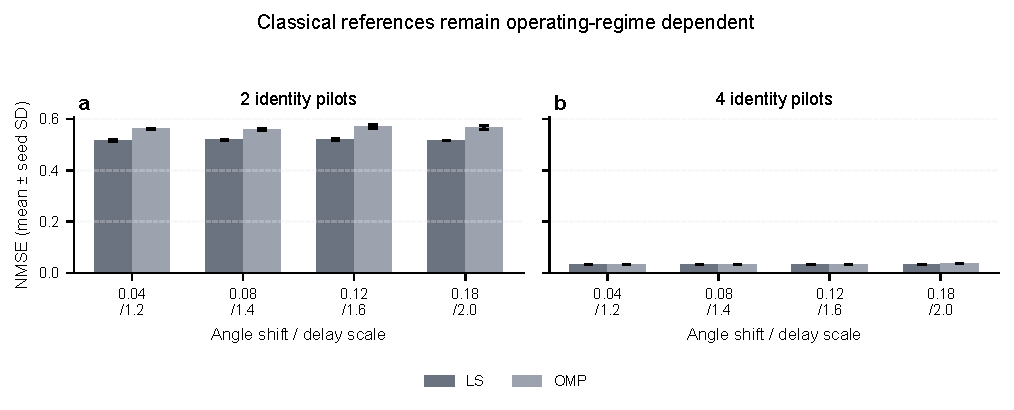
\includegraphics[width=0.86\textwidth]{fig3_classical_sensitivity.pdf}
\caption{\textbf{Classical references and pilot sensitivity.} Fixed-dictionary OMP and LS are evaluated on the explicit RIS generator at 15 dB SNR. Bars show the mean across three seeds and error bars show the standard deviation of seed means. The two-pilot regime is the low-observation setting used by the learned estimator; the four-pilot panel is a separate reference showing how the classical inverse problem changes when all four transmit-antenna columns are observed.}
\label{fig:classical}
\end{figure*}

\begin{table*}[t]
\centering
\caption{Explicit-RIS classical references. Values are mean (SD) across three seeds; the fixed spatial dictionary is used by OMP.}
\label{tab:r032omp}
\begin{tabular}{cccrr}
\toprule
Angle shift & Delay scale & Pilots & LS NMSE & OMP NMSE\\
\midrule
0.04 & 1.2 & 2 & 0.5166 (0.0030) & 0.5621 (0.0011)\\
0.04 & 1.2 & 4 & 0.0316 (0.0001) & 0.0330 (0.0001)\\
0.08 & 1.4 & 2 & 0.5189 (0.0007) & 0.5590 (0.0040)\\
0.08 & 1.4 & 4 & 0.0316 (0.0002) & 0.0331 (0.0001)\\
0.12 & 1.6 & 2 & 0.5193 (0.0037) & 0.5711 (0.0060)\\
0.12 & 1.6 & 4 & 0.0316 (0.0001) & 0.0337 (0.0002)\\
0.18 & 2.0 & 2 & 0.5161 (0.0008) & 0.5684 (0.0071)\\
0.18 & 2.0 & 4 & 0.0318 (0.0001) & 0.0352 (0.0002)\\
\bottomrule
\end{tabular}
\end{table*}


\subsection{Held-out target blocks preserve the recovery direction}

The strict support/evaluation protocol tests whether the canonical result is an artifact of evaluating on the same target batches used to fit the adapter. For each of the three shifts $(0.08,1.4)$, $(0.12,1.6)$ and $(0.18,2.0)$, a 512-realization support block is used for the unlabeled update and a disjoint 512-realization evaluation block is used for scoring. The seeds are separated, the adapter never receives evaluation features or labels during fitting, and the full-model control uses the same split.

The held-out capacity table shows that adapter-only NMSE is lower than frozen NMSE at all three shifts. The mean values are 0.4845 versus 0.4899, 0.5188 versus 0.5245 and 0.5517 versus 0.5616. The paired uncertainty table reports negative adapter-minus-frozen differences for every seed and shift. For example, at $(0.18,2.0)$ the three seed-level differences are approximately $-0.00933$, $-0.00939$ and $-0.00976$, with bootstrap intervals entirely below zero in the recorded evaluation blocks. These intervals support a within-protocol recovery statement. They do not make the result independent of the simulator or prove that the same effect will hold on measured channels.

The held-out result is consequently interpreted at two levels. At the block level, every recorded shift and seed has a negative adapter-minus-frozen difference, so the direction is not driven by a single favorable seed. At the population level, however, the independent unit remains the seed and the generator defines the target population. The intervals quantify paired variation within each evaluation block; they are not a license to generalize beyond the tested simulator or to treat the 3,072 paired observations as 3,072 independent experiments. This distinction is why the paper reports the numerical interval and its unit together.

Full-model adaptation is more accurate in the same held-out control. Its mean NMSE is 0.4807, 0.5043 and 0.5243 at the three shifts, compared with adapter-only values of 0.4845, 0.5188 and 0.5518. The improvement is obtained by updating 115,328 parameters rather than 16,576. Full-model BER is also lower in the recorded rows. Thus, the lightweight adapter should be described as a lower-capacity option with measurable recovery, not as an accuracy-equivalent substitute for full-model updating.

\begin{table*}[t]
\centering
\caption{Held-out capacity control. Values are mean (SD) across three CPU seeds; target labels are not used for adaptation.}
\label{tab:r017}
\resizebox{\textwidth}{!}{%
\begin{tabular}{ccrrrrrr}
\toprule
Angle & Delay & Frozen NMSE & Adapter NMSE & Full NMSE & Adapter BER & Full BER & Full SE\\
shift & scale & & & & & & (bit/s/Hz)\\
\midrule
0.08 & 1.4 & 0.4899 (0.0006) & 0.4845 (0.0003) & 0.4807 (0.0005) & 0.0238 (0.0008) & 0.0175 (0.0014) & 5.6219 (0.0008)\\
0.12 & 1.6 & 0.5245 (0.0010) & 0.5188 (0.0010) & 0.5043 (0.0002) & 0.0283 (0.0015) & 0.0204 (0.0012) & 5.5538 (0.0009)\\
0.18 & 2.0 & 0.5616 (0.0018) & 0.5518 (0.0015) & 0.5243 (0.0010) & 0.0342 (0.0008) & 0.0217 (0.0014) & 5.4915 (0.0030)\\
\bottomrule
\end{tabular}
}
\end{table*}

The complete seed-by-shift paired intervals and Wilcoxon values are provided in Supplementary Table~S2. They are retained for auditability but are not repeated as a second main-text display.

\subsection{Robustness reveals a small-RIS beam-squint failure cell}

The fixed-two-pilot robustness sweep varies RIS size, beam squint and SNR over 18 cells. Figure~\ref{fig:robustness} displays the adapted-minus-frozen deltas for NMSE, BER and spectral efficiency. Negative NMSE and BER deltas favor adaptation; positive spectral-efficiency deltas favor adaptation. Most cells have the expected sign. Without beam squint, all RIS sizes and SNRs show negative NMSE and BER deltas, and the largest RIS has the strongest average NMSE reduction. With beam squint enabled, the effect is smaller and more heterogeneous.

The clearest failure is the eight-element, beam-squint, 5 dB cell. Its NMSE delta is $+0.00176$, its BER delta is $+0.00142$, and its spectral-efficiency delta is $-0.00608$. The adapter worsens all three reported outcomes in that cell, and only one of the three seeds improves NMSE. At eight elements and 25 dB, NMSE and BER are slightly improved but spectral efficiency still falls by $-0.00312$. These rows are not discarded as outliers. They show that a target-pilot objective can be insufficient when the surface aperture and frequency-dependent steering jointly reduce the information available to the adapter.

The same table also shows why the conditional wording matters. At 16 and 32 elements with beam squint, the adapter improves NMSE and BER across all three SNR values, but the spectral-efficiency gain is small at 5 dB and becomes more visible at higher SNR. This is a deployment trade-off, not a monotonic theorem. Geometry, beam squint and SNR jointly determine whether an NMSE change propagates to the communication layer.

The heatmap is therefore read as an operating envelope rather than an average win rate. The non-improving 8-element, 5-dB beam-squint cell is retained because it changes the interpretation of the canonical gain, while the remaining cell-level values are supporting heterogeneity. The full table records all 18 combinations, including the two cells in which spectral efficiency falls despite a small NMSE improvement. These cases matter because a receiver or transmitter responds to the beamformed effective channel, not to NMSE in isolation.

\begin{figure*}[t]
\centering
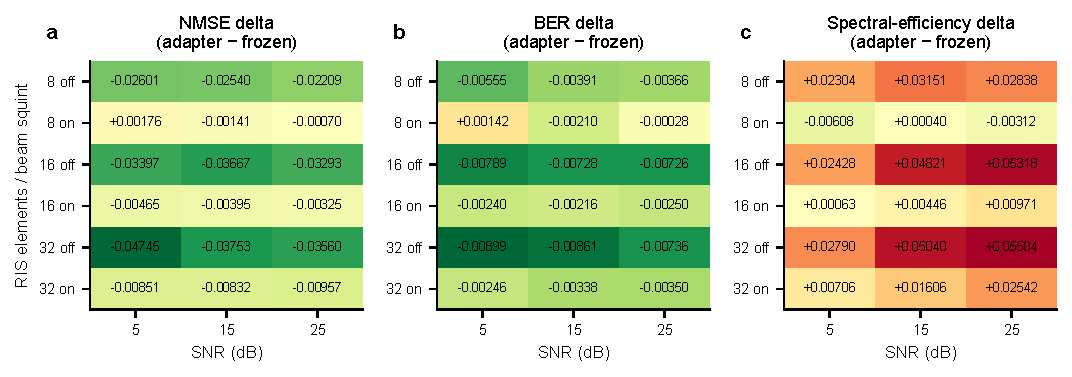
\includegraphics[width=0.98\textwidth]{fig5_robustness.pdf}
\caption{\textbf{Robustness and failure boundaries.} Each heatmap reports the adapted-minus-frozen mean across three seeds for a fixed two-pilot protocol; cell labels are rounded to five decimal places. Negative NMSE and BER deltas favor adaptation; positive spectral-efficiency deltas favor adaptation. The six rows combine RIS size and beam-squint state, and columns are SNR values. The eight-element beam-squint, 5 dB cell is the explicit non-improving control retained in the main evidence chain.}
\label{fig:robustness}
\end{figure*}

The complete 18-cell matrix is provided in Supplementary Table~S3; the main figure and the explicit failure-cell values above carry the conclusion-changing evidence.

\subsection{The preregistered physical term fails its independent-contribution gate}

The physical-control experiment asks whether the tested delay-tail objective adds information beyond pilot consistency and the adapter capacity. It compares no-physics, first-difference and delay-tail objectives on two representative shifts with held-out target blocks and three seeds. The primary paired outcome pools 3,072 channel-level pairs across those blocks; this count is descriptive and does not represent 3,072 independent experiments. The delay-tail minus no-physics NMSE difference is $+0.000885$ with a 95\% bootstrap interval of $[+0.000710,+0.001078]$. Because the interval is positive, the delay-tail objective is worse under the preregistered direction of improvement and fails the independent-contribution gate.

This negative result changes the interpretation of the adapter. The observed recovery is consistent with fitting measurement residuals through a small residual module and with the capacity of the learned estimator. It is not evidence that the fixed delay-tail term captures a necessary wideband propagation mechanism. The first-difference term is retained as a regularizer in the main adapter configuration because it was part of the locked protocol, but the manuscript does not attribute the overall gain to that term. The negative control is included to show how a plausible physical penalty can fail when its effect is tested on hidden target CSI.

\begin{table}[t]
\centering
\caption{Preregistered physical-objective control.}
\label{tab:r021}
\begin{tabular}{lr}
\toprule
Paired samples & 3072\\
Delay-tail $-$ no-physics NMSE & 0.000885\\
Bootstrap 95\% CI & [0.000710, 0.001078]\\
Independent-contribution gate & FAIL\\
\bottomrule
\end{tabular}
\end{table}


\subsection{Accuracy and adaptation cost are separate design axes}

The local CPU profile recorded three wall-clock repeats for label-free adapter-only and full-model updates after the objective was aligned across the two modes. The adapter-only mean was 0.0494 s and the full-model mean was 0.0651 s in this run; the values are hardware-specific measurements rather than a platform-independent speed claim. Device metadata and the exact repeats are retained in the JSON artifact. No CUDA timing is reported in this local package because the current environment has no CUDA device.

The parameter difference is more stable as a design fact than the hardware timing. The adapter updates 16,576 parameters, whereas full-model adaptation updates 115,328, approximately 6.96 times as many. Figure~\ref{fig:cost} therefore separates capacity from timing. A deployment designer may prefer the small adapter when the update memory or model mutability is constrained, while a designer who prioritizes target-domain NMSE may choose full-model updating. The data do not justify collapsing this choice into a single ranking.

The cost comparison also clarifies what is and is not meant by ``lightweight.'' It refers to the number of parameters that are changed during target-time adaptation, not to a claim that the adapter is faster on every device or that it has no accuracy cost. Parameter count and label isolation are more portable design facts; runtime should be remeasured when the model, compiler, batch size or accelerator changes.

\begin{figure*}[t]
\centering
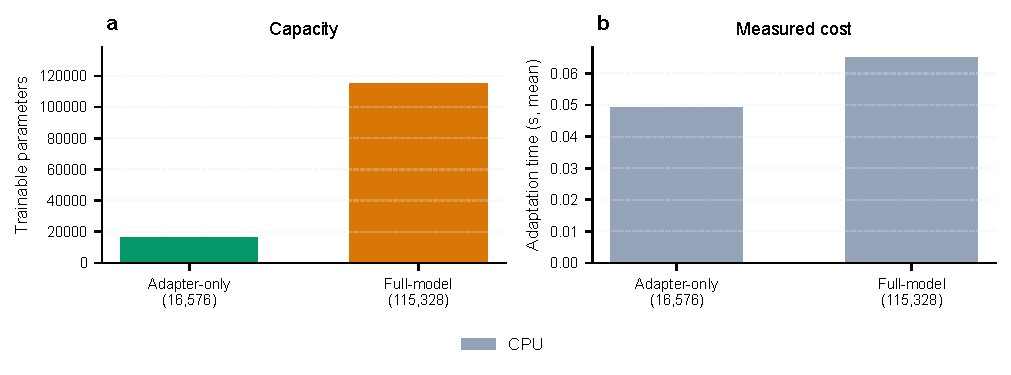
\includegraphics[width=0.82\textwidth]{fig4_capacity_cost.pdf}
\caption{\textbf{Adaptation capacity and measured cost.} The capacity panel reports the trainable parameter counts in the two label-free update modes. The cost panel reports mean wall-clock time over three CPU repeats from the local reproducibility run. Timing is hardware-specific metadata; the figure separates capacity from measured cost and does not establish a hardware-independent runtime ranking. Held-out NMSE values are reported in Table~\ref{tab:r017}.}
\label{fig:cost}
\end{figure*}

\begin{table}[t]
\centering
\caption{Label-free adaptation cost. Wall-clock values are mean (SD) over three CPU repeats.}
\label{tab:r024}
\resizebox{\columnwidth}{!}{%
\begin{tabular}{lrr}
\toprule
Method & Parameters & CPU seconds\\
\midrule
Adapter-only & 16576 & 0.0494 (0.0110)\\
Full-model & 115328 & 0.0651 (0.0091)\\
\bottomrule
\end{tabular}
}
\end{table}


\section{Discussion}

The central finding is that source-free pilot adaptation can recover part of the loss of a frozen learned estimator under explicit wideband RIS shifts, but the evidence supports a protocol-level and conditional interpretation. The canonical sweep, disjoint support/evaluation test, capacity comparison and robustness map jointly distinguish target-time recovery from same-batch fitting, model capacity and geometry-dependent failure. This separation is the main reason to retain both the held-out result and the eight-element beam-squint failure cell in the argument.

The benchmark extends label-free RIS and online-estimation work by making the target information boundary and the downstream consequence visible in one evaluation chain. Self-supervised and zero-shot approaches motivate using target observations without complete labels, while wideband and physics-informed studies motivate exposing angular, delay and beam-squint factors. The present evidence connects these concerns at the protocol level; it does not establish a new universal estimator or replace measured-channel validation.

The communication metrics give the recovery a bounded engineering meaning. The adapter can improve BER and spectral efficiency in the canonical sweep, yet LS remains competitive and can have lower BER. Full-model updating buys lower held-out NMSE at about 6.96 times the trainable parameter count. A deployment choice therefore depends on pilot conditioning, target-block size, available update capacity and the cost of modifying the estimator. The tested delay-tail objective provides a useful counterexample: its positive paired NMSE difference means that a plausible physical penalty did not add independent benefit in this protocol. A different physical constraint would require a new preregistered comparison.

The resulting decision surface is deliberately narrow. Adaptation is most defensible when the source estimator has a measurable target loss and the geometry is outside the observed small-RIS beam-squint failure regime; LS or a sparse method remains a credible fallback when the pilot operator is well conditioned or the residual objective is unstable. These implications concern the tested two-pilot synthetic generator. A measured or ray-traced channel collection with the same support/evaluation split is the next discriminating test because it would determine whether the recovery direction transports beyond the normalized simulator.

\section{Limitations and Conclusion}

The study uses controlled synthetic channels. The generator contains explicit cascaded structure, reflection phases and beam squint, but it does not establish performance on measured RIS hardware, calibration errors, mutual coupling or a site-specific ray-tracing dataset. The canonical sweep uses target-batch adaptation, while the strict support/evaluation result covers three of the four shift levels. The conclusion about held-out transport should therefore be read over the tested held-out shifts rather than extended to every possible target environment.

The learned estimator and adapter are compact multilayer perceptrons. CNN, transformer and large-scale model-based estimators are outside the current comparison, and OMP uses a fixed dictionary rather than a fully tuned SBL implementation. The classical baseline is therefore informative about the tested operating regime but does not exhaust model-based alternatives. The CPU cost measurement is tied to the local software and hardware environment and should be remeasured for another deployment. The search boundary is also explicit. Five neighboring DOI records were verified, but broad keyword services were partly rate limited, so the manuscript does not issue a global novelty certificate.

These limitations affect transportability rather than the internal accounting of the reported simulator experiments. The next discriminating test is a measured or ray-traced channel collection that preserves the same support/evaluation isolation, pilot budget, shift metadata and paired seed logic. If the recovery direction survives that test, the benchmark would support a stronger deployment claim. If it does not, the present results would still identify which simulator factors overstate the value of pilot-only updates. The experiment is therefore a resolution of a named uncertainty, rather than a generic request for more data.

Within these boundaries, the study establishes a reproducible benchmark for source-free pilot adaptation under explicit RIS wideband distribution shifts. The adapter recovers a frozen estimator on the canonical sweep and on disjoint held-out blocks, but its gains depend on geometry, beam squint, SNR and adaptation capacity. The OMP and LS controls show that pilot budget changes the classical operating regime, the full-model control shows the cost of capacity, and the negative physical control prevents an unsupported mechanism claim. The scientific value of the result lies in making those conditions visible and reproducible. A next decisive experiment is measured-channel or ray-traced validation with the same support/evaluation isolation, because that test would determine whether the observed recovery is transportable beyond the controlled generator.

\section*{Data availability}

The study uses synthetic wideband BS--RIS--UE channel realizations generated by the scripts in the accompanying project bundle. The generator, fixed configurations, seeds, JSON result summaries, table exporters, figure source, CPU-loadable model weights and verification manifests are publicly available at \url{https://github.com/pengliangtian06-commits/ris-source-free-pilot-adaptation/tree/v1.0.3}. The v1.0.3 release is archived at Zenodo under version DOI \url{https://doi.org/10.5281/zenodo.23121462}. The package contains synthetic data and does not claim public measured-channel data availability.

\section*{Code and model availability}

Source code is released under the MIT License. Manuscript text, figures, tables, generated result artifacts and model weights are released under CC BY 4.0. The weights are plain CPU-loadable \texttt{state\_dict} files with JSON metadata and were verified with \texttt{weights\_only=True}; no executable objects or target CSI labels are stored in the weights. The local timing records are hardware-specific and are not a platform-independent benchmark.

\section*{Declaration of competing interests}

The authors declare that they have no known competing financial interests or personal relationships that could have appeared to influence this work.

\section*{Funding}

This research received no specific grant from any funding agency in the public, commercial or not-for-profit sectors.

\section*{Acknowledgements}

There are no additional acknowledgements. No human participants, animals or personally identifiable data are involved.

\section*{Author contributions: CRediT}

Pengliang Tian: Conceptualization, Methodology, Software, Investigation, Data curation, Writing -- original draft. Changjiang Zhang: Supervision, Validation, Writing -- review and editing. Changjiang Zhang is the corresponding author (zhangchangjiang@ccbupt.cn).

\section*{Declaration of generative AI and AI-assisted technologies in the manuscript preparation process}

During preparation of this manuscript, AI-assisted tools were used for research-workflow organization, language editing, code--paper consistency checks and draft revision support. The authors designed the study, controlled the experiments, inspected the source artifacts, verified the quantitative claims and take full responsibility for the final manuscript and its contents. No AI system is listed as an author.

\bibliographystyle{IEEEtranN}
\bibliography{references}
\end{document}
